\documentclass[a4]{article}
\pagestyle{myheadings}

%%%%%%%%%%%%%%%%%%%
% Packages/Macros %
%%%%%%%%%%%%%%%%%%%
\usepackage{mathrsfs}


\usepackage{fancyhdr}
\pagestyle{fancy}
\lhead{}
\chead{}
\rhead{}
\lfoot{}
\cfoot{} 
\rfoot{\normalsize\thepage}
\renewcommand{\headrulewidth}{0pt}
\renewcommand{\footrulewidth}{0pt}
\newcommand{\RomanNumeralCaps}[1]
    {\MakeUppercase{\romannumeral #1}}

\usepackage{amssymb,latexsym}  % Standard packages
\usepackage[utf8]{inputenc}
\usepackage[russian]{babel}
\usepackage{MnSymbol}
\usepackage{mathrsfs}
\usepackage{amsmath,amsthm}
\usepackage{indentfirst}
\usepackage{graphicx}%,vmargin}
\usepackage{graphicx}
\graphicspath{{pictures/}} 
\usepackage{verbatim}
\usepackage{color}
\usepackage{color,colortbl}
\usepackage[nottoc,numbib]{tocbibind}
\usepackage{float}
\usepackage{multirow}
\usepackage{hhline}

\usepackage{listings}
\definecolor{codegreen}{rgb}{0,0.6,0}
\definecolor{codegray}{rgb}{1,1,1}
\definecolor{codepurple}{rgb}{0.58,0,0.82}
\definecolor{backcolour}{rgb}{0.95,0.95,0.92}
 
\lstdefinestyle{mystyle}{
    backgroundcolor=\color{backcolour},   
    commentstyle=\color{codegreen},
    keywordstyle=\color{magenta},
    numberstyle=\tiny\color{codegray},
    stringstyle=\color{codepurple},
    basicstyle=\footnotesize,
    breakatwhitespace=false,         
    breaklines=true,                 
    captionpos=b,                    
    keepspaces=true,                 
    numbers=left,                    
    numbersep=5pt,                  
    showspaces=false,                
    showstringspaces=false,
    showtabs=false,                  
    tabsize=2
}
 
\lstset{style=mystyle}

\usepackage{url}
\urldef\myurl\url{foo%.com}
\def\UrlBreaks{\do\/\do-}
\usepackage{breakurl}
\Urlmuskip=0mu plus 1mu



\DeclareGraphicsExtensions{.pdf,.png,.jpg}% -- настройка картинок

\usepackage{epigraph} %%% to make inspirational quotes.
\usepackage[all]{xy} %for XyPic'a
\usepackage{color} 
\usepackage{amscd} %для коммутативных диграмм
%\usepackage[colorlinks,urlcolor=red]{hyperref}

%\renewcommand{\baselinestretch}{1.5}
%\sloppy
%\usepackage{listings}
%\lstset{numbers=left}
%\setmarginsrb{2cm}{1.5cm}{1cm}{1.5cm}{0pt}{0mm}{0pt}{13mm}


\newtheorem{Lemma}{Лемма}[section]
\newtheorem{Proposition}{Предложение}[section]
\newtheorem{Theorem}{Теорема}[section]
\newtheorem{Corollary}{Следствие}[section]
\newtheorem{Remark}{Замечание}[section]
\newtheorem{Definition}{Определение}[section]
\newtheorem{Designations}{Обозначение}[section]




%%%%%%%%%%%%%%%%%%%%%%% 
%Подготовка оглавления% 
%%%%%%%%%%%%%%%%%%%%%%% 
\usepackage[titles]{tocloft}
\renewcommand{\cftdotsep}{2} %частота точек
\renewcommand\cftsecleader{\cftdotfill{\cftdotsep}}
\renewcommand{\cfttoctitlefont}{\hspace{0.38\textwidth} \LARGE\bfseries} 
\renewcommand{\cftsecaftersnum}{.}
\renewcommand{\cftsubsecaftersnum}{.}
\renewcommand{\cftbeforetoctitleskip}{-1em} 
\renewcommand{\cftaftertoctitle}{\mbox{}\hfill \\ \mbox{}\hfill{\footnotesize Стр.}\vspace{-0.5em}} 
%\renewcommand{\cftchapfont}{\normalsize\bfseries \MakeUppercase{\chaptername} } 
%\renewcommand{\cftsecfont}{\hspace{1pt}} 
\renewcommand{\cftsubsecfont}{\hspace{1pt}} 
%\renewcommand{\cftbeforechapskip}{1em} 
\renewcommand{\cftparskip}{3mm} %определяет величину отступа в оглавлении
\setcounter{tocdepth}{5} 
\renewcommand{\listoffigures}{\begingroup %добавляем номер в список иллюстраций
\tocsection
\tocfile{\listfigurename}{lof}
\endgroup}
\renewcommand{\listoftables}{\begingroup %добавляем номер в список иллюстраций
\tocsection
\tocfile{\listtablename}{lot}
\endgroup}


%\renewcommand{\thelikesection}{(\roman{likesection})}
%%%%%%%%%%%
% Margins %
%%%%%%%%%%%
\addtolength{\textwidth}{0.7in}
\textheight=630pt
\addtolength{\evensidemargin}{-0.4in}
\addtolength{\oddsidemargin}{-0.4in}
\addtolength{\topmargin}{-0.4in}

%%%%%%%%%%%%%%%%%%%%%%%%%%%%%%%%%%%
%%%%%%Переопределение chapter%%%%%% 
%%%%%%%%%%%%%%%%%%%%%%%%%%%%%%%%%%%
\newcommand{\empline}{\mbox{}\newline} 
\newcommand{\likechapterheading}[1]{ 
\begin{center} 
\textbf{\MakeUppercase{#1}} 
\end{center} 
\empline} 

%%%%%%%Запиливание переопределённого chapter в оглавление%%%%%% 
\makeatletter 
\renewcommand{\@dotsep}{2} 
\newcommand{\l@likechapter}[2]{{\bfseries\@dottedtocline{0}{0pt}{0pt}{#1}{#2}}} 
\makeatother 
\newcommand{\likechapter}[1]{ 
\likechapterheading{#1} 
\addcontentsline{toc}{likechapter}{\MakeUppercase{#1}}} 




\usepackage{xcolor}
\usepackage{hyperref}
\definecolor{linkcolor}{HTML}{000000} % цвет ссылок
\definecolor{urlcolor}{HTML}{3643FF} % цвет гиперссылок
 
\hypersetup{pdfstartview=FitH,  linkcolor=linkcolor,urlcolor=urlcolor, colorlinks=true}

%%%%%%%%%%%%
% Document %
%%%%%%%%%%%%

%%%%%%%%%%%%%%%%%%%%%%%%%%%%%
%%%%%%главы -- section*%%%%%%
%%%%section -- subsection%%%%
%subsection -- subsubsection%
%%%%%%%%%%%%%%%%%%%%%%%%%%%%%
\def \newstr {\medskip \par \noindent} 



\begin{document}
\newcolumntype{g}{>{\columncolor{codegray}}c}



\def\contentsname{\LARGE{Содержание}}
\thispagestyle{empty}
\begin{center} 
	\vspace{2cm} 
	{\Large \sc Санкт-Петербургский Политехнический Университет}\\
	\vspace{2mm}
	{\Large\sc им. Петра Великого}\\
	\vspace{1cm}
	{\large \sc Институт прикладной математики и механики\\ 
		\vspace{0.5mm}
		\textsc{}}\\ 
	\vspace{0.5mm}
	{\large\sc Кафедра $"$Прикладная математика$"$}\\
	\vspace{15mm}
	
	
	{\sc \textbf{Отчёт\\
			Лабораторная работа № 6\\
			по дисциплине\\
			"Математическая статистика"}
		\vspace{6mm}
		
	}
	\vspace*{2mm}
	
	
	\begin{flushleft}
		\vspace{4cm}
		\sc Выполнил студент:\\
		\sc Шарапов Сергей Андреевич\\
		\sc группа: 3630102/70401\\
		\vspace{1cm}
		\sc Проверил:\\
		\sc к.ф-м.н., доцент\\
		\sc Баженов Александр Николаевич
		\vspace{20mm}
	\end{flushleft}
\end{center} 
\begin{center}
	\vfill {\large\textsc{Санкт-Петербург}}\\ 
	2020 год
\end{center}

%%%%%%%%%%%%%%%%%%%%%%%%%%%%%%%%%%%%%%%%%%%%%%%%%%%%%%%%%%%%%%%%%%%%%%%%%%%%%%%%%%%%%%%%%%%%%%
%\ \\[4cm]

%\rm
%%%%%%%%%%%%%%%%%%%%%%%%%%%%%%%%%%%%%%%%%%%%%%%%%%%%%%%%%%%%%%%%%%%%%%%%%%%%%%%%%%%%%%%%%%%%%%
\newpage
\pagestyle{plain}

%\begin{center}
%\begin{abstract} 

%\end{abstract}

%\end{center}

\newpage
\tableofcontents{}
\newpage
\listoffigures{}
\listoftables{}
\newpage

\section{Постановка задачи}

Необходимо найти оценки линейной регрессии $y_i=a+bx_i+e_i,$ используя $20$ точек отрезка $[-1.8;\;2]$ с равномерным шагом $0.2.$ Ошибку $e_i$ считать нормально распределённой с параметрами $(0,\;1).$ В качестве эталонной зависимости взять $y_i=2+2x_i+e_i.$ При построении оценок коэффициентов использовать два критерия: критерий наименьших квадратов и критерий наименьших модулей.

Проделать то же самое для выборки, у которой в значении $y_1$ и $y_{20}$ вносятся возмущения $10$ и $-10$ соответственно.

\section{Теория}
Простая линейная регрессия \cite{lin_reg}:
\begin{equation}
    y_i=ax_i+b+e_i,\;i=\overline{1,n},\hfill
\end{equation}

где $x_i\;\--$ заданные числа, $y_i\;\--$ наблюдаемые значения отклика, $e_i\;\--$ независимые, нормально распределённые с нулевым математическим ожиданием и одинаковой (неизвестной) дисперсией случайные величины (ненаблюдаемые), $a$ и $b\;\--$ неизвестные параметры, подлежащие оцениванию.

\subsection{Метод наименьших квадратов}

Критерий $\--$ минимизация функции \cite{MNK}:
\begin{equation}
    Q(a,b)=\sum\limits_{i=1}^n(y_i-ax_i-b)^2\to \min\hfill
\end{equation}

Оценка $\overset{\wedge}{a}$ и $\overset{\wedge}{b}$ параметров $a$ и $b,$ в которых достигается минимум $Q(a,b),$ называются МНК-оценками. Формулы для их вычисления:
\begin{equation}
    \begin{cases}
    \overset{\wedge}{a} = \frac{\overline{x y}-\overline{x}\overline{y}}{\overline{x^2}-\overline{x}^2}\\
    \overset{\wedge}{b} = \overline{y}-\overset{\wedge}{a}\overline{x}
    \end{cases}\hfill
\end{equation}

Оценка по методу наименьших квадратов является несмещённой оценкой.

МНК чувствителен к выбросам (т.к. в вычислении используется выборочное среднее, значение которого крайне неустойчиво к большим по относительной величине выбросам)

\subsection{Метод наименьших модулей}
Критерий наименьших модулей – заключается в минимизации следующей функции \cite{6_4}:
\begin{equation}
    M(a,b) = \sum\limits_{i=1}^n\vert y_i-ax_i-b\vert\to\min\hfill
\end{equation}

Формулы для вычисления робастных параметров:
\begin{equation}
\begin{cases}
&  \hat{a}_{R} = r_{Q}\frac{q_{y}^{*}}{q_{x}^{*}} \\ 
&  \hat{b}_{R}= medy - \hat{a}_{R}medx
\end{cases}
\end{equation}, где 
\begin{equation}
	r_{Q} = \frac{1}{n}\sum sgn(x_{i} - medx)sgn(y_{i} - medy)
\end{equation}

Статистики выборочной медианы и интерквартильной широты обладают
робастными свойствами в силу того, что основаны на центральных порядковых статистиках, малочувствительных к большим по величине выбросам
в данных. Статистика выборочного знакового коэффициента корреляции
робастна, так как знаковая функция $ sgn z $ чувствительна не к величине
аргумента, а только к его знаку. Отсюда оценка МНМ обладает очевидными робастными свойствами устойчивости к выбросам по
координате $ y $, но она довольно груба.

\section{Реализация}
Работы была выполнена на языке $Python 3.8.2$
Для генерации выборок использовался модуль $numpy$.
Для построения графиков использовалась библиотека $matplotlib$.
Регрессионные модели использовались из библиотеки $statsmodels$.

\section{Результаты}

%\vspace{-2cm}
\begin{figure}[H]
    \centering
    \caption{Графики линейной регрессии}
    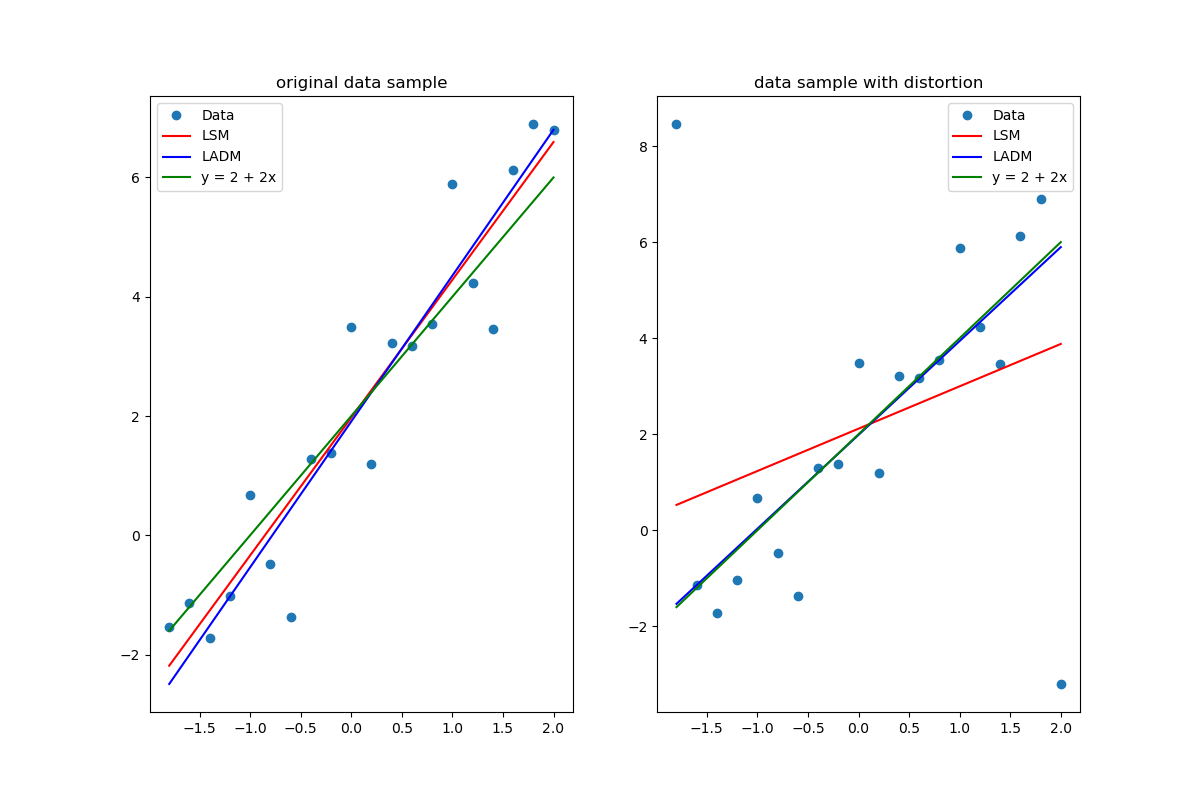
\includegraphics[scale = 0.6]{graph.png} 
    \label{fig:reg}
\end{figure}

\begin{table}[H]
\caption{Таблица оценок коэффициентов линейной регрессии без возмущёний}
\label{tab:my_label1}
\begin{center}
\vspace{5mm}
\begin{tabular}{|c|c|c|}
\hline
& $\overset{\wedge}{a}$ & $\overset{\wedge}{b}$\\
\hline
МНК &1.739737&1.924716\\
\hline
МНМ &1.935446&1.742526\\
\hline
\end{tabular}
\end{center}
\end{table}


\begin{table}[H]
\caption{Таблица оценок коэффициентов линейной регрессии с возмущёниями}
\label{tab:my_label2}
\begin{center}
\vspace{5mm}
\begin{tabular}{|c|c|c|}
\hline
& $\overset{\wedge}{a}$ & $\overset{\wedge}{b}$\\
\hline
МНК &0.311165&2.067573\\
\hline
МНМ &1.877536 &1.707785\\
\hline
\end{tabular}
\end{center}
\end{table}



\section{Выводы}
По графику видно, что оба метода дают хорошую оценку коэффициентов линейной регрессии, при отсутствии выбросов. Однако выбросы сильно влияют на оценки по МНК.

Выбросы мало влияют на оценку по МНМ, но ценой за это является б\'oльшая по сравнению с МНК сложность вычисления. На практике зачастую легче просто отсеять выбросы из выборки.


\section{Литература}

\href{https://physics.susu.ru/vorontsov/language/numpy.html}{Модуль numpy}\\

\href{https://matplotlib.org/}{Модуль matplotlib}\\

\href{https://www.scipy.org/}{Модуль scipy}\\

Шевляков Г. Л. Лекции по математической статистике, 2019.


\section{Приложения}

\href{https://github.com/Sergey-Sharapov/MatStat_labs/blob/main/lab6/lab6.py}{Код лабораторной}


\end{document}
